\begin{figure*}[t]
    \centering
    \begin{minipage}{0.4975\textwidth}
        \centering
        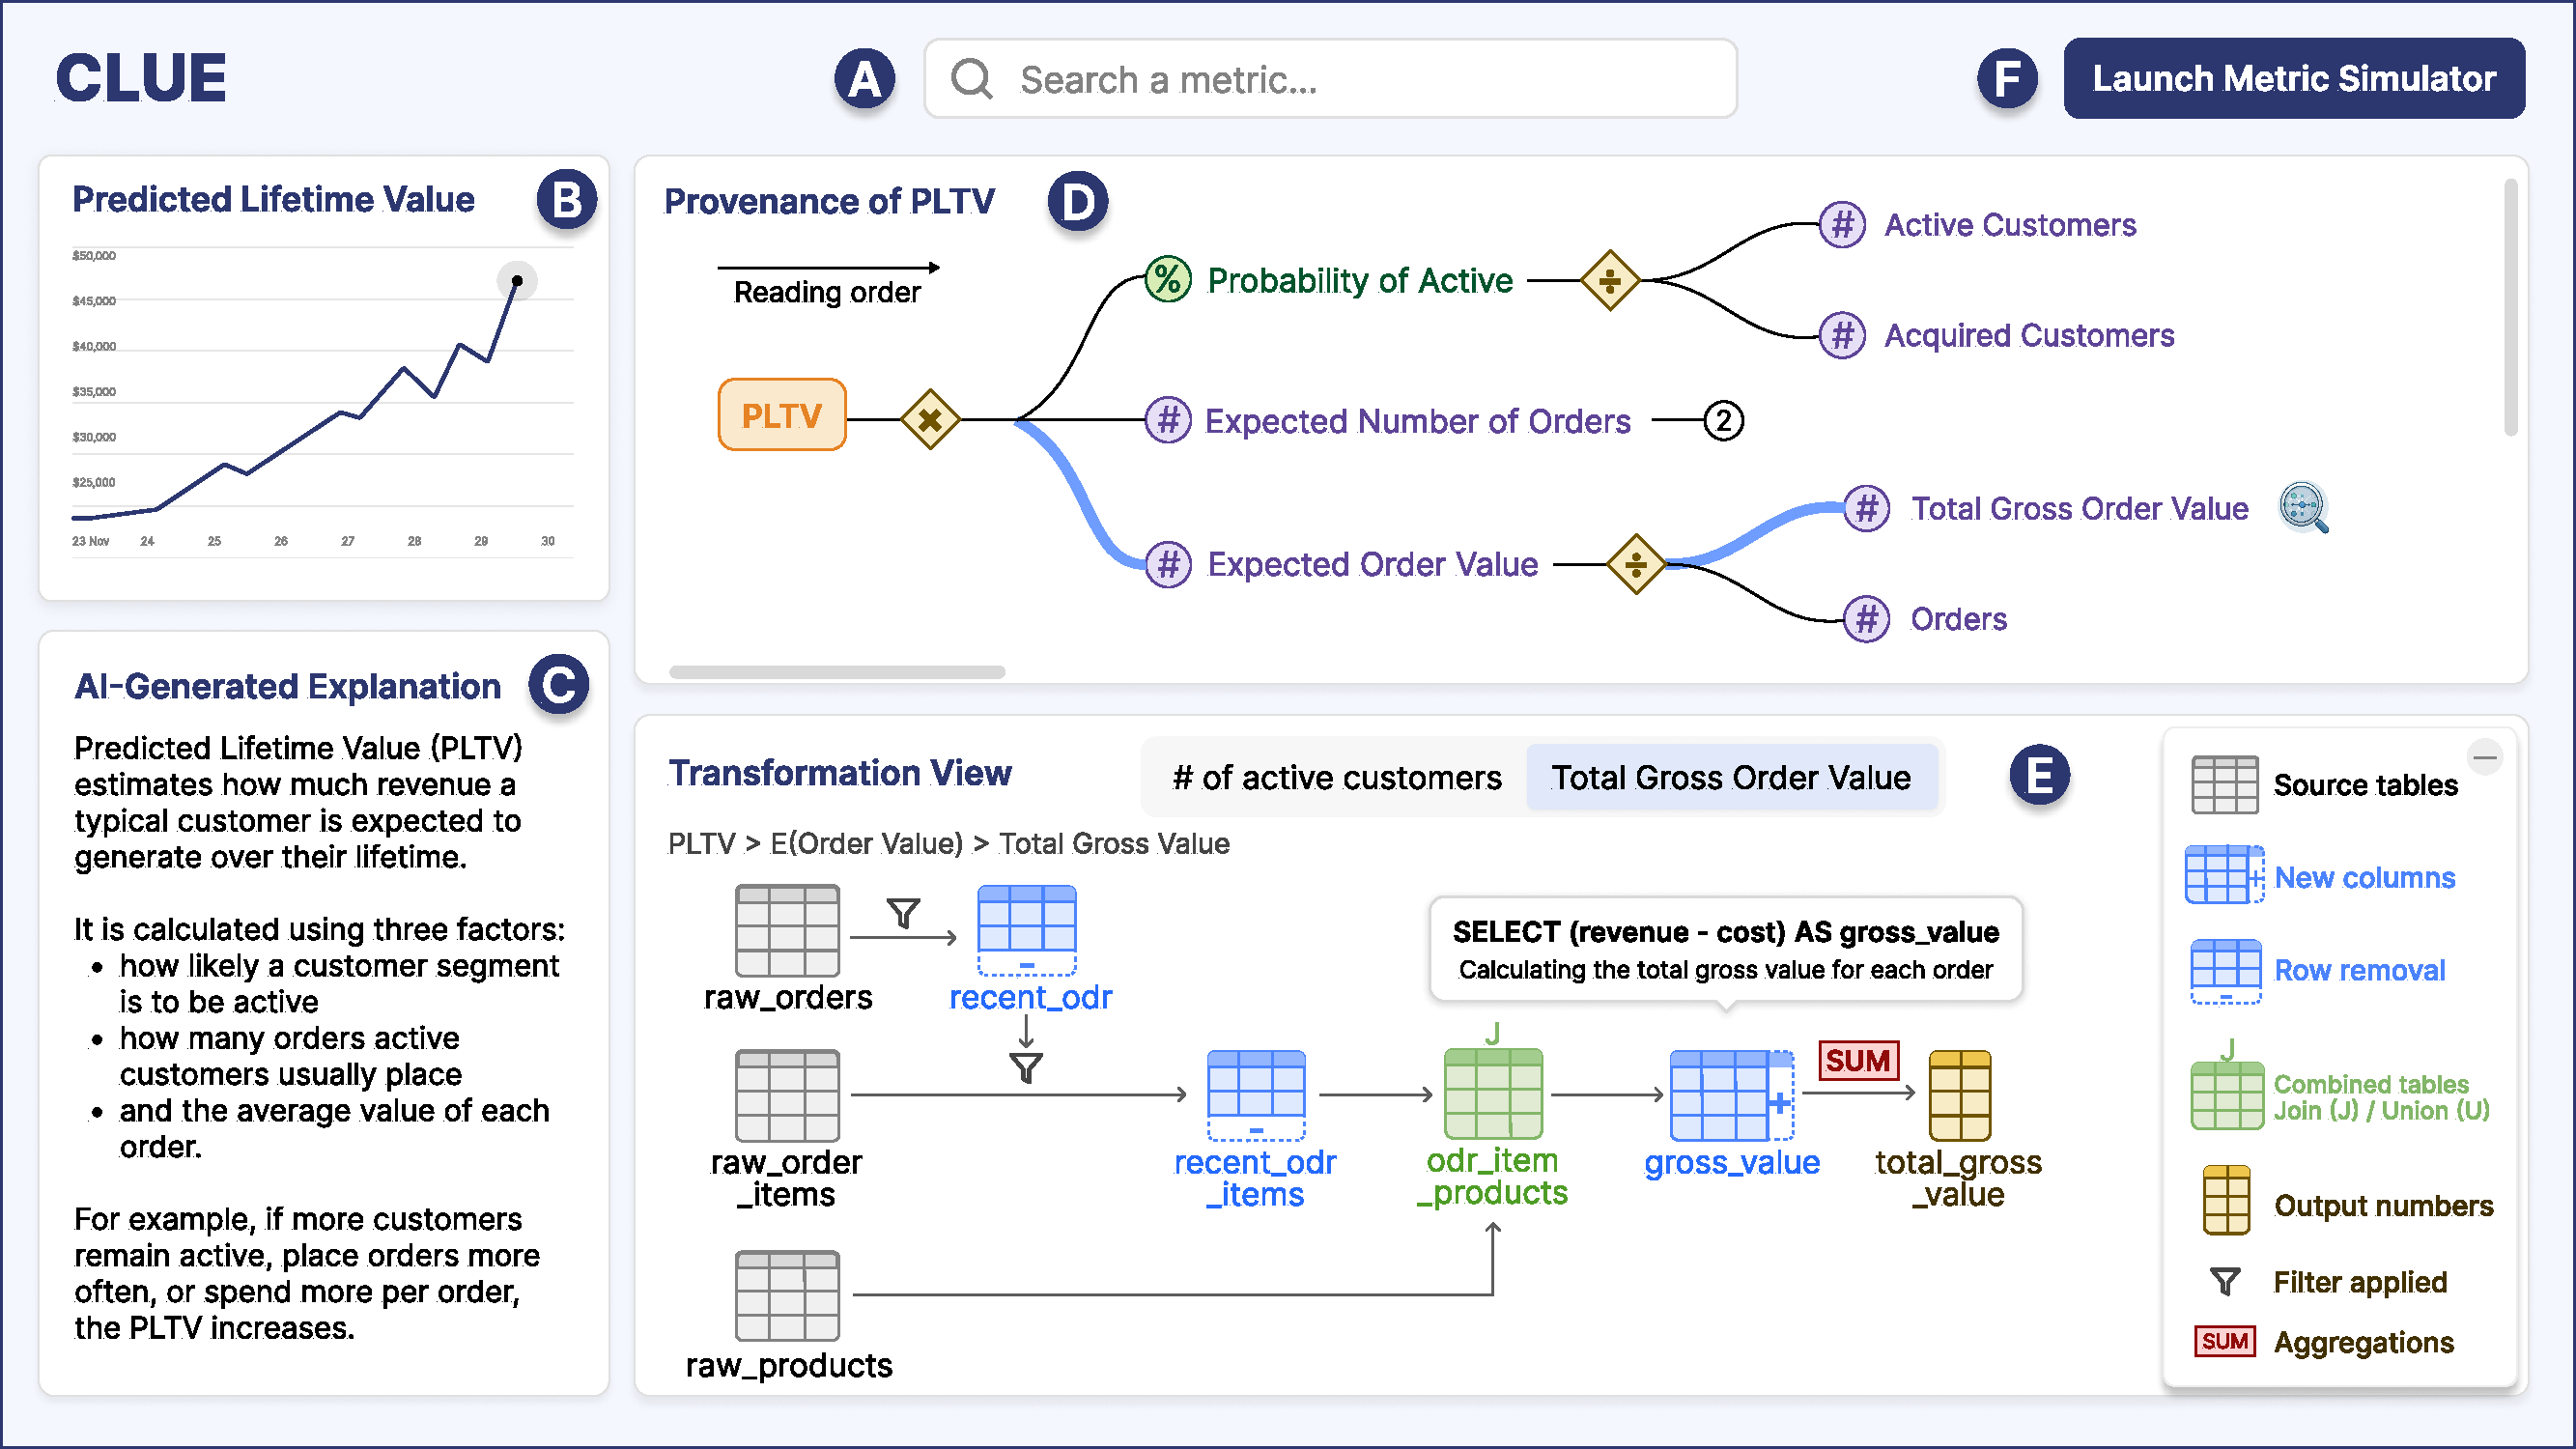
\includegraphics[width=\textwidth,page=1]{figures/UI Wireframe - metric provenance.pdf}
    \end{minipage}
    \hfill
    \begin{minipage}{0.4975\textwidth}
        \centering
        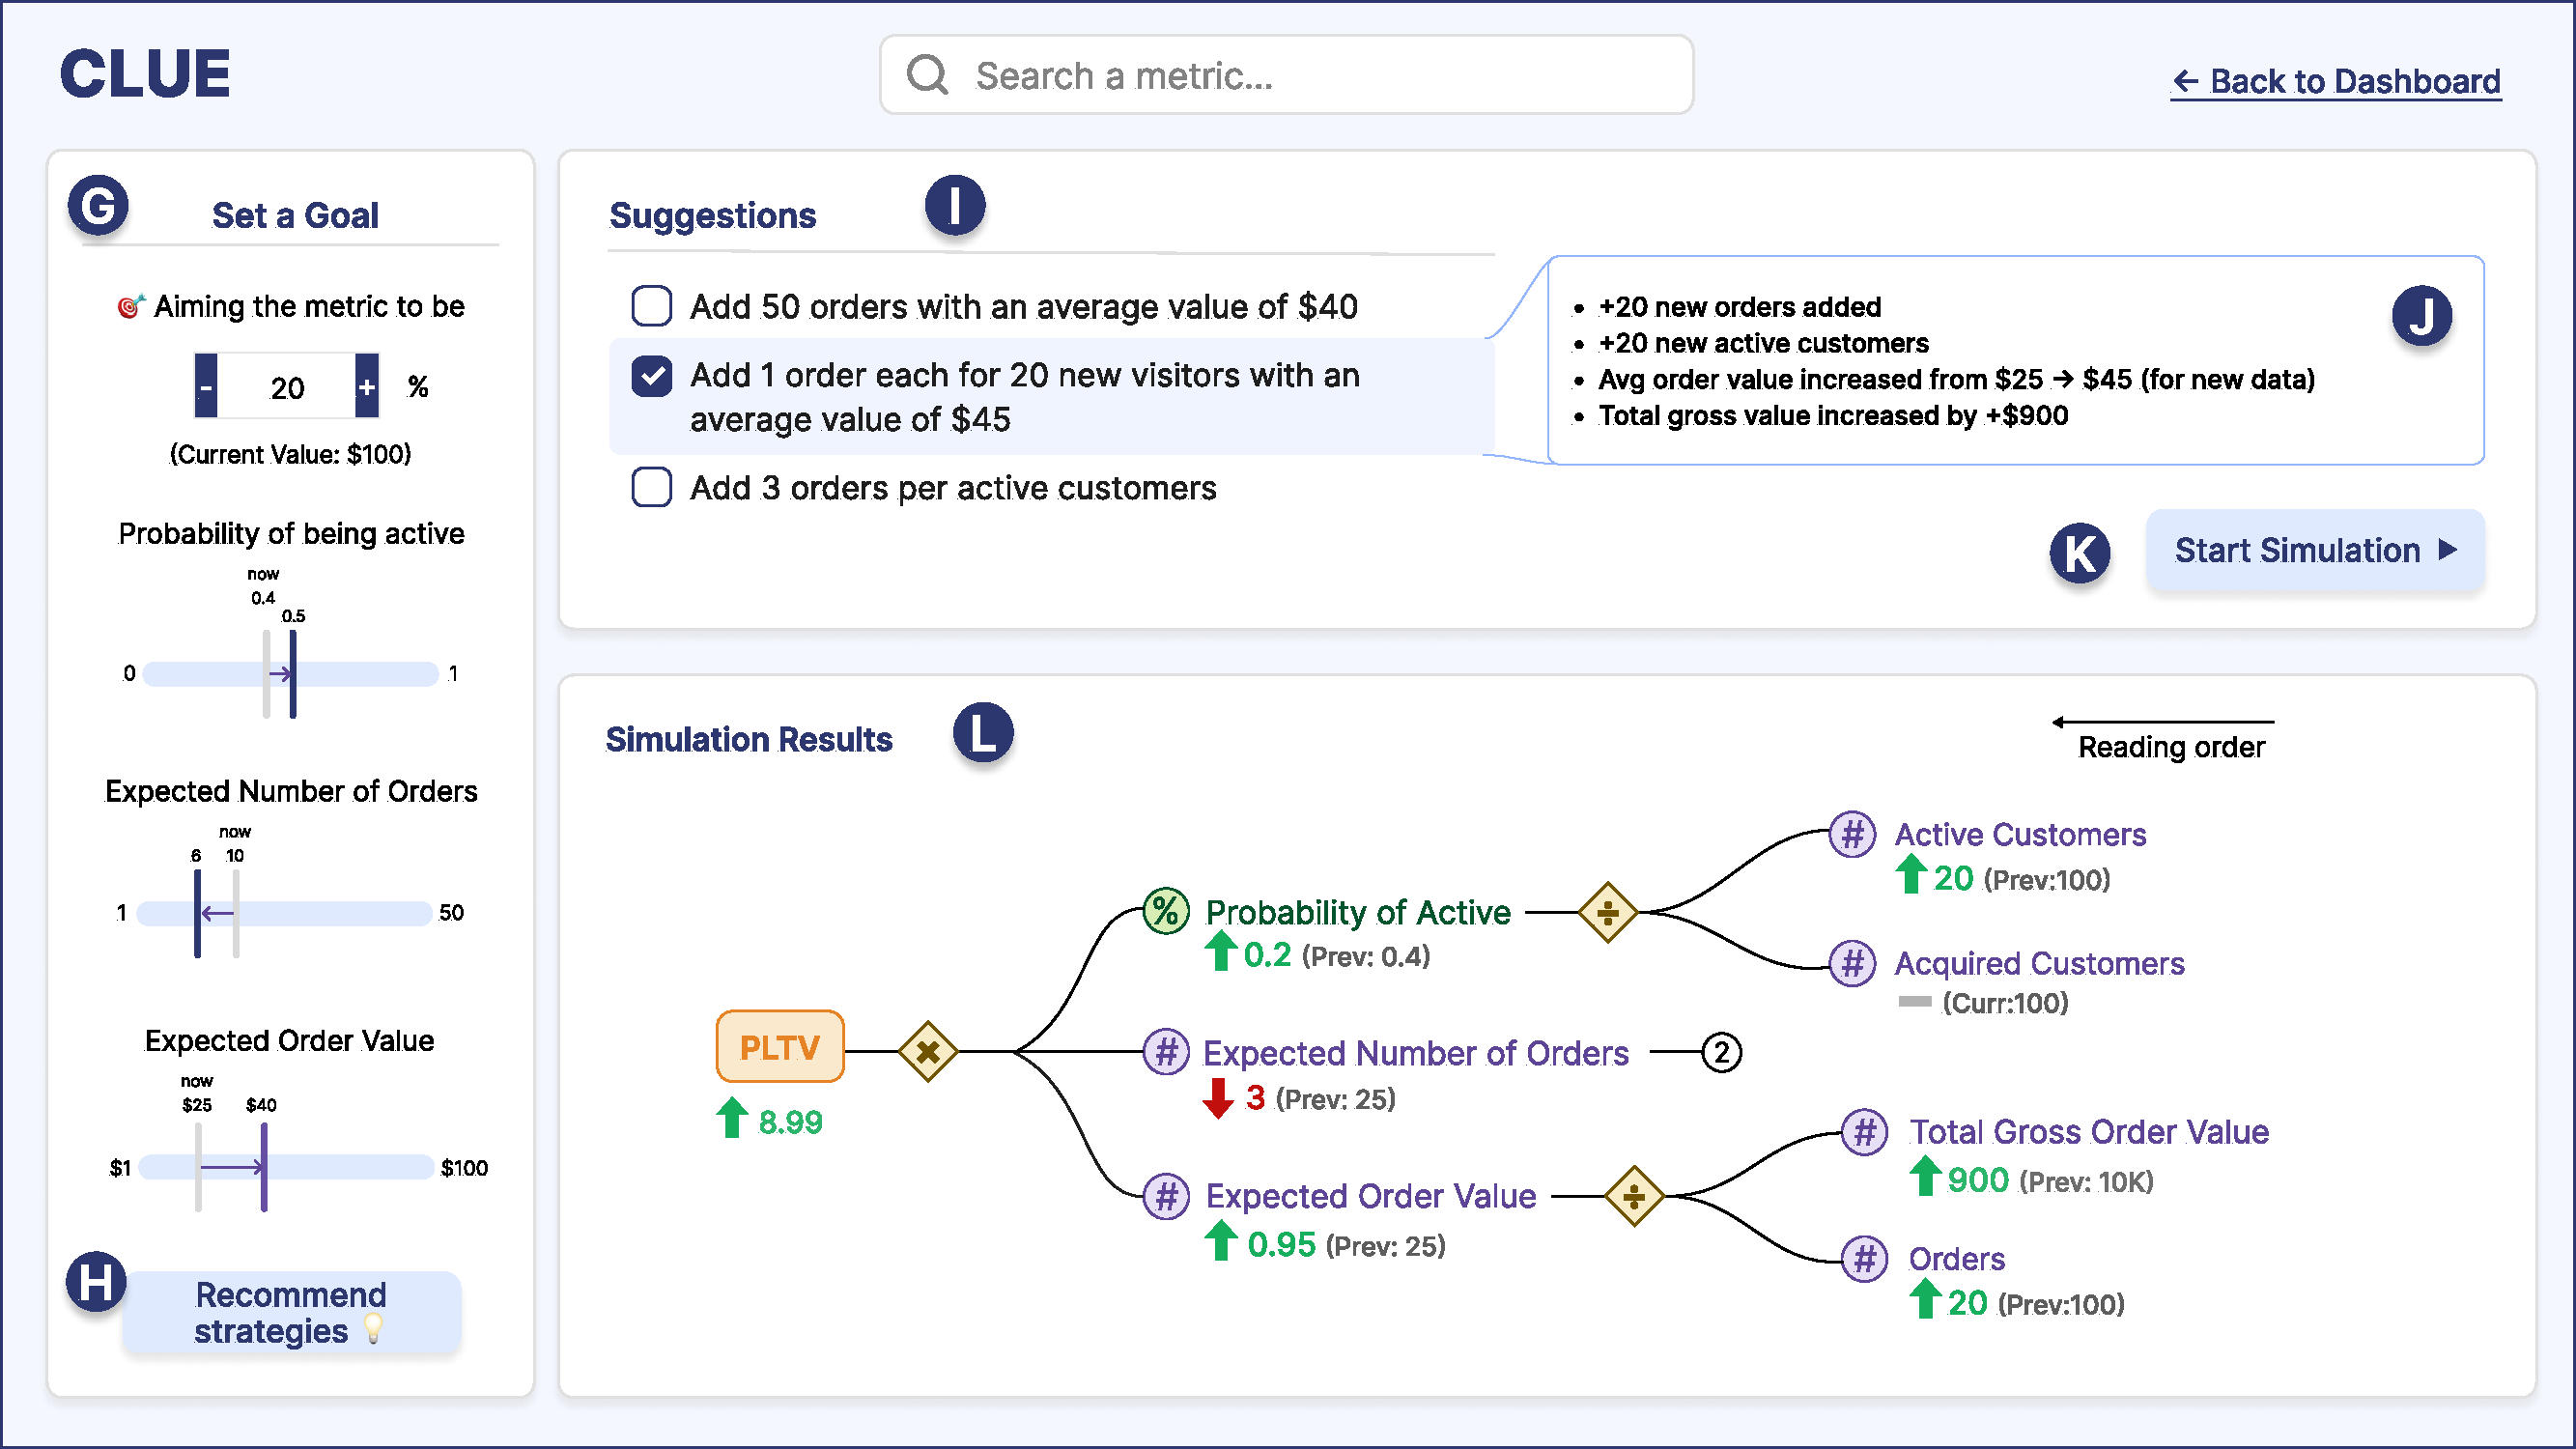
\includegraphics[width=\textwidth,page=1]{figures/UI Wireframe - metric simulator.pdf}
    \end{minipage}
    % 
\includegraphics[width=1\linewidth]{VLDB 2026 Demo//figures/UI Wireframe - metric provenance.pdf}

    {\scriptsize sample scriptsize text}
    \caption{
	\small
	The \clue interface:
    \stepCounter{A} search for a metric, 
    \stepCounter{B} CLUE presents the trend of the metric,
    \stepCounter{C} CLUE generates metric explanation,
    \stepCounter{D} CLUE extracts and visualize metric lineages,
    \stepCounter{E} CLUE extracts and visualize data transformation processes,
    \stepCounter{F} launch the Metric Simulator,
    \stepCounter{G} set up a target number of the metric and tune the desired number for each first-level submetrics,
    \stepCounter{H} generate suggestions to achieve the goal,
    \stepCounter{I} view and select a suggestion, \stepCounter{J} view the data adjustment summary,
    \stepCounter{J} start simulation,
    \stepCounter{K} CLUE computes and presents the value changes on each metric.
    }
\label{clue}
\end{figure*}